\documentclass[a4paper]{article}

\usepackage[pdftex,
 hidelinks,
 pdfauthor={Dexter Chua},
 pdfsubject={Cambridge Maths Notes: Part IB - Metric and Topological Spaces},
 pdftitle={Part IB - Metric and Topological Spaces},
pdfkeywords={Cambridge Mathematics Maths Math IB Easter Metric Topological Spaces}]{hyperref}

\title{Part IB - Metric and Topological Spaces}
\author{Lectured by J. Rasmussen}
\date{Easter 2015}

% Imports
\ifx \nextra \undefined
  \usepackage[pdftex,
    hidelinks,
    pdfauthor={Dexter Chua},
    pdfsubject={Cambridge Maths Notes: Part \npart\ - \ncourse},
    pdftitle={Part \npart\ - \ncourse},
  pdfkeywords={Cambridge Mathematics Maths Math \npart\ \nterm\ \nyear\ \ncourse}]{hyperref}
  \title{Part \npart\ - \ncourse}
\else
  \usepackage[pdftex,
    hidelinks,
    pdfauthor={Dexter Chua},
    pdfsubject={Cambridge Maths Notes: Part \npart\ - \ncourse\ (\nextra)},
    pdftitle={Part \npart\ - \ncourse\ (\nextra)},
  pdfkeywords={Cambridge Mathematics Maths Math \npart\ \nterm\ \nyear\ \ncourse\ \nextra}]{hyperref}

  \title{Part \npart\ - \ncourse \\ {\Large \nextra}}
\fi

\author{Lectured by \nlecturer \\\small Notes taken by Dexter Chua}
\date{\nterm\ \nyear}

\usepackage{alltt}
\usepackage{amsfonts}
\usepackage{amsmath}
\usepackage{amssymb}
\usepackage{amsthm}
\usepackage{booktabs}
\usepackage{caption}
\usepackage{enumitem}
\usepackage{fancyhdr}
\usepackage{graphicx}
\usepackage{mathtools}
\usepackage{microtype}
\usepackage{multirow}
\usepackage{pdflscape}
\usepackage{pgfplots}
\usepackage{siunitx}
\usepackage{tabularx}
\usepackage{tikz}
\usepackage{tkz-euclide}
\usepackage[normalem]{ulem}
\usepackage[all]{xy}

\pgfplotsset{compat=1.12}

\pagestyle{fancyplain}
\lhead{\emph{\nouppercase{\leftmark}}}
\ifx \nextra \undefined
  \rhead{
    \ifnum\thepage=1
    \else
      \npart\ \ncourse
    \fi}
\else
  \rhead{
    \ifnum\thepage=1
    \else
      \npart\ \ncourse\ (\nextra)
    \fi}
\fi
\usetikzlibrary{arrows}
\usetikzlibrary{decorations.markings}
\usetikzlibrary{decorations.pathmorphing}
\usetikzlibrary{positioning}
\usetikzlibrary{fadings}
\usetikzlibrary{intersections}
\usetikzlibrary{cd}

\newcommand*{\Cdot}{\raisebox{-0.25ex}{\scalebox{1.5}{$\cdot$}}}
\newcommand {\pd}[2][ ]{
  \ifx #1 { }
    \frac{\partial}{\partial #2}
  \else
    \frac{\partial^{#1}}{\partial #2^{#1}}
  \fi
}

% Theorems
\theoremstyle{definition}
\newtheorem*{aim}{Aim}
\newtheorem*{axiom}{Axiom}
\newtheorem*{claim}{Claim}
\newtheorem*{cor}{Corollary}
\newtheorem*{defi}{Definition}
\newtheorem*{eg}{Example}
\newtheorem*{fact}{Fact}
\newtheorem*{law}{Law}
\newtheorem*{lemma}{Lemma}
\newtheorem*{notation}{Notation}
\newtheorem*{prop}{Proposition}
\newtheorem*{thm}{Theorem}

\renewcommand{\labelitemi}{--}
\renewcommand{\labelitemii}{$\circ$}
\renewcommand{\labelenumi}{(\roman{*})}

\let\stdsection\section
\renewcommand\section{\newpage\stdsection}

% Strike through
\def\st{\bgroup \ULdepth=-.55ex \ULset}

% Maths symbols
\newcommand{\bra}{\langle}
\newcommand{\ket}{\rangle}

\newcommand{\N}{\mathbb{N}}
\newcommand{\Z}{\mathbb{Z}}
\newcommand{\Q}{\mathbb{Q}}
\renewcommand{\H}{\mathbb{H}}
\newcommand{\R}{\mathbb{R}}
\newcommand{\C}{\mathbb{C}}
\newcommand{\Prob}{\mathbb{P}}
\renewcommand{\P}{\mathbb{P}}
\newcommand{\E}{\mathbb{E}}
\newcommand{\F}{\mathbb{F}}
\newcommand{\cU}{\mathcal{U}}
\newcommand{\RP}{\mathbb{RP}}
\newcommand{\CP}{\mathbb{CP}}

\newcommand{\ph}{\,\cdot\,}

\DeclareMathOperator{\sech}{sech}
\DeclareMathOperator{\cosech}{cosech}
\DeclareMathOperator{\cosec}{cosec}

\DeclareMathOperator{\covol}{covol}
\DeclareMathOperator{\vol}{vol}

\let\Im\relax
\let\Re\relax
\DeclareMathOperator{\Im}{Im}
\DeclareMathOperator{\Re}{Re}
\DeclareMathOperator{\im}{im}
\DeclareMathOperator{\image}{image}
\DeclareMathOperator{\Ann}{Ann}

\DeclareMathOperator*{\res}{res}
\DeclareMathOperator{\Res}{Res}
\DeclareMathOperator{\Ind}{Ind}

\DeclareMathOperator{\tr}{tr}
\DeclareMathOperator{\diag}{diag}
\DeclareMathOperator{\rank}{rank}
\DeclareMathOperator{\card}{card}
\DeclareMathOperator{\spn}{span}
\DeclareMathOperator{\adj}{adj}

\DeclareMathOperator{\erf}{erf}
\DeclareMathOperator{\erfc}{erfc}

\DeclareMathOperator{\ord}{ord}
\DeclareMathOperator{\Sym}{Sym}

\DeclareMathOperator{\sgn}{sgn}
\DeclareMathOperator{\orb}{orb}
\DeclareMathOperator{\stab}{stab}
\DeclareMathOperator{\ccl}{ccl}

\DeclareMathOperator{\lcm}{lcm}
\DeclareMathOperator{\hcf}{hcf}

\DeclareMathOperator{\Int}{Int}
\DeclareMathOperator{\id}{id}

\DeclareMathOperator{\betaD}{beta}
\DeclareMathOperator{\gammaD}{gamma}
\DeclareMathOperator{\Poisson}{Poisson}
\DeclareMathOperator{\binomial}{binomial}
\DeclareMathOperator{\multinomial}{multinomial}
\DeclareMathOperator{\Bernoulli}{Bernoulli}
\DeclareMathOperator{\like}{like}

\DeclareMathOperator{\var}{var}
\DeclareMathOperator{\cov}{cov}
\DeclareMathOperator{\bias}{bias}
\DeclareMathOperator{\mse}{mse}
\DeclareMathOperator{\corr}{corr}

\DeclareMathOperator{\otp}{otp}
\DeclareMathOperator{\dom}{dom}

\DeclareMathOperator{\Root}{Root}
\DeclareMathOperator{\supp}{supp}
\DeclareMathOperator{\rel}{rel}
\DeclareMathOperator{\Hom}{Hom}
\DeclareMathOperator{\Aut}{Aut}
\DeclareMathOperator{\Gal}{Gal}
\DeclareMathOperator{\Mat}{Mat}
\DeclareMathOperator{\End}{End}
\DeclareMathOperator{\Char}{char}
\DeclareMathOperator{\ev}{ev}
\DeclareMathOperator{\St}{St}
\DeclareMathOperator{\Lk}{Lk}
\DeclareMathOperator{\disc}{disc}
\DeclareMathOperator{\Isom}{Isom}
\DeclareMathOperator{\length}{length}
\DeclareMathOperator{\energy}{energy}
\DeclareMathOperator{\area}{area}
\DeclareMathOperator{\Syl}{Syl}
\DeclareMathOperator{\cl}{cl}
\DeclareMathOperator{\fix}{fix}

\newcommand{\GL}{\mathrm{GL}}
\newcommand{\SL}{\mathrm{SL}}
\newcommand{\PGL}{\mathrm{PGL}}
\newcommand{\PSL}{\mathrm{PSL}}
\newcommand{\PSU}{\mathrm{PSU}}
\newcommand{\Or}{\mathrm{O}}
\newcommand{\SO}{\mathrm{SO}}
\newcommand{\U}{\mathrm{U}}
\newcommand{\SU}{\mathrm{SU}}

\renewcommand{\d}{\mathrm{d}}
\newcommand{\D}{\mathrm{D}}

\tikzset{->/.style = {decoration={markings,
                                  mark=at position 1 with {\arrow[scale=2]{latex'}}},
                      postaction={decorate}}}
\tikzset{<-/.style = {decoration={markings,
                                  mark=at position 0 with {\arrowreversed[scale=2]{latex'}}},
                      postaction={decorate}}}
\tikzset{<->/.style = {decoration={markings,
                                   mark=at position 0 with {\arrowreversed[scale=2]{latex'}},
                                   mark=at position 1 with {\arrow[scale=2]{latex'}}},
                       postaction={decorate}}}
\tikzset{->-/.style = {decoration={markings,
                                   mark=at position #1 with {\arrow[scale=2]{latex'}}},
                       postaction={decorate}}}
\tikzset{-<-/.style = {decoration={markings,
                                   mark=at position #1 with {\arrowreversed[scale=2]{latex'}}},
                       postaction={decorate}}}

\tikzset{circ/.style = {fill, circle, inner sep = 0, minimum size = 3}}
\tikzset{mstate/.style={circle, draw, blue, text=black, minimum width=0.7cm}}

\definecolor{mblue}{rgb}{0.2, 0.3, 0.8}
\definecolor{morange}{rgb}{1, 0.5, 0}
\definecolor{mgreen}{rgb}{0.1, 0.4, 0.2}
\definecolor{mred}{rgb}{0.5, 0, 0}

\def\drawcirculararc(#1,#2)(#3,#4)(#5,#6){%
    \pgfmathsetmacro\cA{(#1*#1+#2*#2-#3*#3-#4*#4)/2}%
    \pgfmathsetmacro\cB{(#1*#1+#2*#2-#5*#5-#6*#6)/2}%
    \pgfmathsetmacro\cy{(\cB*(#1-#3)-\cA*(#1-#5))/%
                        ((#2-#6)*(#1-#3)-(#2-#4)*(#1-#5))}%
    \pgfmathsetmacro\cx{(\cA-\cy*(#2-#4))/(#1-#3)}%
    \pgfmathsetmacro\cr{sqrt((#1-\cx)*(#1-\cx)+(#2-\cy)*(#2-\cy))}%
    \pgfmathsetmacro\cA{atan2(#2-\cy,#1-\cx)}%
    \pgfmathsetmacro\cB{atan2(#6-\cy,#5-\cx)}%
    \pgfmathparse{\cB<\cA}%
    \ifnum\pgfmathresult=1
        \pgfmathsetmacro\cB{\cB+360}%
    \fi
    \draw (#1,#2) arc (\cA:\cB:\cr);%
}
\newcommand\getCoord[3]{\newdimen{#1}\newdimen{#2}\pgfextractx{#1}{\pgfpointanchor{#3}{center}}\pgfextracty{#2}{\pgfpointanchor{#3}{center}}}

\def\Xint#1{\mathchoice
   {\XXint\displaystyle\textstyle{#1}}%
   {\XXint\textstyle\scriptstyle{#1}}%
   {\XXint\scriptstyle\scriptscriptstyle{#1}}%
   {\XXint\scriptscriptstyle\scriptscriptstyle{#1}}%
   \!\int}
\def\XXint#1#2#3{{\setbox0=\hbox{$#1{#2#3}{\int}$}
     \vcenter{\hbox{$#2#3$}}\kern-.5\wd0}}
\def\ddashint{\Xint=}
\def\dashint{\Xint-}


\begin{document}
\maketitle
{\small
\noindent\textbf{Metrics}\\
Definition and examples. Limits and continuity. Open sets and neighbourhoods. Characterizing limits and continuity using neighbourhoods and open sets.\hspace*{\fill} [3]

\vspace{10pt}
\noindent\textbf{Topology}\\
Definition of a topology. Metric topologies. Further examples. Neighbourhoods, closed sets, convergence and continuity. Hausdorff spaces. Homeomorphisms. Topological and non-topological properties. Completeness. Subspace, quotient and product topologies.\hspace*{\fill} [3]

\vspace{10pt}
\noindent\textbf{Connectedness}\\
Definition using open sets and integer-valued functions. Examples, including intervals. Components. The continuous image of a connected space is connected. Path-connectedness. Path-connected spaces are connected but not conversely. Connected open sets in Euclidean space are path-connected.\hspace*{\fill} [3]

\vspace{10pt}
\noindent\textbf{Compactness}\\
Definition using open covers. Examples: finite sets and [0, 1]. Closed subsets of compact spaces are compact. Compact subsets of a Hausdorff space must be closed. The compact subsets of the real line. Continuous images of compact sets are compact. Quotient spaces. Continuous real-valued functions on a compact space are bounded and attain their bounds. The product of two compact spaces is compact. The compact subsets of Euclidean space. Sequential compactness.\hspace*{\fill} [3]}

\tableofcontents
\setcounter{section}{-1}
\section{Introduction}
In Analysis, we defined a lot of things for real numbers. For example, if $(x_n)$ is a sequence in $\R$, $x_n \to x$ if
\[
  (\forall \varepsilon > 0)(\exists N)(\forall n > N) |x_n - x| < \varepsilon.
\]
$f: \R \to \R$ is said to be continuous iff $f(x_n) \to f(x)$ whenever $x_n \to x$.

How can we make sense of these notions, when we are no longer talking about the reals? For example,
\begin{itemize}
  \item Let $X = \{A \in M_{k\times k}(\R) | A^T = A\}$. Define $F: X\to \R$ to be $F(a) =$ the largest eigenvalue of $A$. Is this continuous?

  \item Let $X = \{f: [0, 1]\to \R: f\text{ is continuous}\}$. Let $F: X \to \R$ map $F(f) = f(\frac{1}{2})$. Is this continuous?
\end{itemize}

We also have a lot of theorems about continuous functions. For example, the intermediate value theorems says that if $f:[0, 1] \to \R$ is continuous, $f(0) < 0$, $f(0) > 0$, then $\exists x\in [0, 1]$ such that $f(x) = 0$.  The maximum value theorem says that if $f:[0, 1] \to \R$ is continuous, $\exists x\in [0, 1]$ such that $f(x) \geq f(y)$ for all $y\in [0, 1]$.

How can we extend these to non-$\R$ spaces?

We will answer these questions in this course.

\section{Metric spaces}
Let $(\mathbf{v}_n) = ((x_n, y_n))$ be a sequence in $\R^2$. What should it mean for $(\mathbf{v}_n) \to \mathbf{v} = (x, y)$.

Intuitively, it should mean $(x_n) \to x$ and $(y_n) \to y$. This is equivalent to saying that $|x_n - x| \to 0$ and $|y_n - y| \to 0$, or $(x_n - x)^2 + (y_n - y)^2 \to 0$. This in turn is equivalent to saying that $|\mathbf{v}_n - \mathbf{v}| \to 0$, where $|\mathbf{v}_n - \mathbf{v}|$ is the Euclidean distance from $\mathbf{v}_n$ to $\mathbf{v}$, defined as $|(x, y)| = \sqrt{x^2 + y^2}$.

So we can define sequence convergence just by considering the distances between points.
\begin{defi}[Metric space]
  A \emph{metric space} is a pair $(X, d_X)$ where $X$ is a set (the space) and $d_X$ is a function $d_X: X \times X \to \R$ (the metric) such that (for all $x, y, z$.
  \begin{itemize}
    \item $d_X(x, y) \geq 0$ (non-negativity)
    \item $d_X(x, y) = 0$ iff $x = y$ (identity of indiscernibles)
    \item $d_X(x, y) = d_X(y, x)$ (symmetry) \item $d_X(x, z) \leq d_X(x, y) + d_X(y, z)$ (triangle inequality)
  \end{itemize}
\end{defi}

\begin{eg}\leavevmode
  \begin{itemize}
    \item Let $X = \R^n$. Let 
      \[
        d(\mathbf{v}, \mathbf{w}) = |\mathbf{v} - \mathbf{w}| = \sqrt{\sum_{i = 1}^n (v_i - w_i)^2}.
      \]
      This is the Euclidean metric.
    \item Let $X$ be a set, and
      \[
        d_X(x, y) =
        \begin{cases}
          1 & x \not= y\\
          0 & x = y
        \end{cases}
      \]
      The first three axioms are trivially satisfied. How about the fourth? The left hand side is either $0$ or $1$, and RHS is 0, 1, 2. It can only possibly fail if RHS = 0, but this means $x = y = z$. So LHS = 0 as well. So we are safe.
  \end{itemize}
\end{eg}
\begin{defi}[Metric subspace]
  Let $(X, d_X)$ be a metric space, and $Y\subseteq X$. Then $(Y, d_Y)$ is a metric space, where $d_Y(a, b) = d_X(a, b)$, and said to be a \emph{subspace} of $X$. 
\end{defi}

\begin{eg}
  For example, $S^n = \{\mathbf{v}\in \R^{n + 1}: |\mathbf{v} = 1\}$, the $n$-dimensional sphere, is a subspace of $\R^{n + 1}$.
\end{eg}

\begin{defi}[Convergent sequences]
  Let $(X_n)$ be a sequence in a metric space $(X, d_X)$. We say $(x_n)$ \emph{converges to} $x\in X$, written $x_n \to x$, if $(d(x_n, x)) \to 0$. Equivalently, 
  \[
    (\forall \varepsilon)(\exists N)(\forall n > N) \to d(x_n, X) < \varepsilon.
  \]
\end{defi}
\begin{eg}\leavevmode
  \begin{itemize}
    \item If $(\mathbf{v}_n)$ is a sequence in $\R^k$ with the Euclidean metric, with $\mathbf{v}_n = (v_n^1, \cdots, v_n^k)$, $v = (v^1, \cdots, v^k)\in \R^k$, then $\mathbf{v}_n \to \mathbf{v}$ iff $(v_n^i) \to v^i$ for all $i$.

    \item If $X$ has the discrete metric, then $x_n \to x$ iff $x_n = x$ for all but finitely many $n$, ie. it is eventually always $x$ (take $\varepsilon = \frac{1}{2}$).
  \end{itemize}
\end{eg}

\begin{prop}
  If $(X, d)$ is a metric place, $(x_n)$ is a sequence in $X$ such that $x_n \to x$, $x_n \to x'$, then $x = x'$.
\end{prop}

\begin{proof}
  Given $\varepsilon > 0$. Then $\exists N$ such that $d(x_n, x) < \varepsilon/2$ if $n > N$, and $\exists N'$ such that $d(x_n, x') < \varepsilon/2$ if $n > N'$. Then if $n > \max(N, N')$, then 
  \begin{align*}
    0 \leq d(x, x') &\leq d(x, x_n) + d(x_n, x')\\
    &= d(x_n, x) + d(x_n, x')\\
    &\leq \varepsilon.
  \end{align*}
  So $0 \leq d(x, x') \leq \varepsilon$ for all $\varepsilon > 0$. So $d(x, x') = 0$, and $x = x'$.

  Note that we used all of the axioms. We used non-negativity when we said $0\leq d(x, x')$. We used the triangle inequality for the next inequality, and symmetry to swap $d(x, x_n)$ with $d(x_n, x)$. Now we use the identity of indiscernibles to say that since $d(x, x') = 0$, they must be equal.
\end{proof}

\begin{defi}[Continuity]
  If $(X, d_X)$ and $(Y, d_Y)$ are metric spaces, and $f:X \to Y$, we say $f$ is \emph{continuous} if $f(x_n) \to f(x)$ (in $Y$) whenever $x_n \to x$ (in $X$).
\end{defi}

\begin{eg}
  Let $X = \R$ with the Euclidean metric. Let $Y = \R$ with the discrete metric. Then
  $f:X \to Y$ that maps $f(x) = x$ is not continuous. This is since $1/n \to 0$ in the Euclidean metric, but not in the discrete metric.
  
  However, $g: Y\to X$ by $g(x) = x$ is continuous, since a sequence in $Y$ that converges is eventually constant.
\end{eg}

\subsection{Examples of metric spaces}
\begin{eg}[Manhattan metric]
  Let $X = \R^2$, and
  \[
    d(\mathbf{x}, \mathbf{y}) = d((x_1, x_2), (y_1, y_2))  = |x_1 - y_1| + |x_2 - y_2|.
  \]
  The first three axioms are again trivial. To prove the triangle inequality, we have
  \begin{align*}
    d(\mathbf{x}, \mathbf{y}) + d(\mathbf{y}, \mathbf{z}) &= |x_1 - y_1| + |x_2 - y_2| + |y_1 - z_1| + |y_2 - z_2|\\
    &\geq |x_1 - z_1| + |z_2 - z_2|\\
    &= d(\mathbf{x}, \mathbf{z}),
  \end{align*}
  using the triangle inequality for $\R$. This is the distance from a point to another where you are only allowed to move horizontally or vertically, but not diagonally.
\end{eg}

\begin{eg}[British railway metric]
  Let $x = \R^2$. We define
  \[
    d(\mathbf{x}, \mathbf{y}) = 
    \begin{cases}
      |\mathbf{x} - \mathbf{y}|&\text{if }\mathbf{x} = k\mathbf{y}\\
      |\mathbf{x}| + |\mathbf{y}|&\text{otherwise}
    \end{cases}
  \]
  To explain the name of this metric, think of Britain with London as the origin. Since the railway system is \st{stupid} less than ideal, all trains go through London. For example, if you want to go from Oxford to Cambridge (and obviously not the other way round), you go from Oxford to London, then London to Cambridge. So the distance traveled is the distance from London to Oxford plus the distance from London to Cambridge.

  The exception is when the two destinations lie along the same line, in which case, you can directly take the train from one to the other without going through London, and hence the ``if $\mathbf{x} = k\mathbf{y}$'' clause.
\end{eg}

\begin{eg}[$p$-adic metric]
  Let $p\in \Z$ be a prime number. Then define
  \[
    |n|_p = 
    \begin{cases}
      p^{-k} & n = p^k m, p\nmid m\\
      0 & n = 0
    \end{cases}
  \]
  Take $X = \Z$, $d_p (a, b) = |a - b|_p$.  Observe that
  \[
    |a - b|_p \leq \max\{|a|_p, |b|_p\}
  \]
  by doing some funny stuff about divisibility. So the triangle inequality follows.

  With respect to $d_2$, we have $1, 2, 4, 8, 16, 32, \cdots \to 0$.
\end{eg}

\begin{eg}[Uniform metric]
  Let $X = C[0, 1]$, the set of all continuous functions on $[0, 1]$. Then define
  \[
    d(f, g) = \max_{x\in [0, 1]}|f(x) - g(x)|
  \]
  which exists since continuous functions are bounded and attains their bounds.

  For example, let $F: C[0, 1] \to \R$ be defined by $F(f) = f(\frac{1}{2})$. Then this is continuous with respect to the uniform metric on $C[0, 1]$ and the usual metric on $\R$.

  If $f_n \to f$ in the uniform metric, then we have to show that $F(f_n) \to F(f)$, ie. $f_n(\frac{1}{2}) \to f(\frac{1}{2})$.

  Let $a_n = |f_n(\frac{1}{2}) - f(\frac{1}{2})|$ and $b_n = \max |f_n(x) - f(x)|$. Then trivially
  \[
    0 \leq a_n \leq b_n \to 0.
  \]
  So $a_n \to 0$. So $f_n(\frac{1}{2}) \to f(\frac{1}{2})$.
\end{eg}

\subsection{Norms}
\begin{defi}[Norm]
  If $V$ is a real vector space, a \emph{norm} on $V$ is a function $\|\cdot \|: V\to \R$ such that
  \begin{itemize}
    \item $\|\mathbf{v}\| \geq 0$ for all $\mathbf{v}\in V$
    \item $\|\mathbf{v}\| = 0$ if and only if $\mathbf{v} = \mathbf{0}$.
    \item $\|\lambda \mathbf{v}\| = |\lambda|\|\mathbf{v}\|$
    \item $\|\mathbf{v} + \mathbf{w}\| \leq \|\mathbf{v}\| + \|\mathbf{w}\|$.
  \end{itemize}
\end{defi}

\begin{eg}
  Let $V = \R^n$. We can let
  \[
    \|\mathbf{v}\|_1 = \sum_{i = 1}^n  |v_i|.
  \]
  We can also let
  \[
    \|\mathbf{v}\|_2 = \sqrt{\sum_{i = 1}^n v_i^2},
  \]
  the \emph{Euclidean norm}.

  Finally, we can have
  \[
    \|\mathbf{v}\|_\infty = \max \{|v_i|: 1 \leq i \leq n\}.
  \]
  In general, we have
  \[
    \|\mathbf{v}\|_p = \left(\sum_{i = 1}^n |v_i|^p\right)^{1/p}.
  \]
  for any $1 \leq p \leq \infty$ is a norm, and $\|\mathbf{v}\|_\infty$ is the limit as $p\to \infty$. 

  Proof that these are norms are left as an exercise for the reader (in the example sheets).
\end{eg}

\begin{lemma}
  If $\|\cdot\|$ is a norm on $V$, then
  \[
    d(\mathbf{v}, \mathbf{w}) = \|\mathbf{v} - \mathbf{w}\|
  \]
  defines a metric on $V$.
\end{lemma}

\begin{proof}\leavevmode
  \begin{enumerate}
    \item $d(\mathbf{v}, \mathbf{w}) = \|\mathbf{v} - \mathbf{w}\| \geq 0$ by the definition of the norm.
    \item $d(\mathbf{v}, \mathbf{w}) = 0 \Leftrightarrow \|\mathbf{v} - \mathbf{w}\} = 0 \Leftrightarrow \mathbf{v} - \mathbf{w} = \mathbf{0} \Leftrightarrow \mathbf{v} = \mathbf{w}$.
    \item $d(\mathbf{w}, \mathbf{v}) = \|\mathbf{w} - \mathbf{v}\| = \|(-1)(\mathbf{v} - \mathbf{w})\| = |-1| \|\mathbf{v} - \mathbf{w}\| = d(\mathbf{v}, \mathbf{w})$.
    \item $d(\mathbf{u}, \mathbf{v}) + d(\mathbf{v}, \mathbf{w}) = \|\mathbf{u} - \mathbf{v}\| + \|\mathbf{v} - \mathbf{w}\| \geq \|\mathbf{u} - \mathbf{w}\| = d(\mathbf{u}, \mathbf{w})$.
  \end{enumerate}
\end{proof}

\begin{defi}[Inner product]
  If $V$ is a real vector space, an \emph{inner product} on $V$ is a function $\bra \cdot, \cdot\ket: V\times V \to \R$ such that
  \begin{enumerate}
    \item $\bra \mathbf{v}, \mathbf{v}\ket \geq 0$ for all $\mathbf{v}\in V$
    \item $\bra \mathbf{v}, \mathbf{v}\ket = 0$ if and only if $\mathbf{v} = \mathbf{0}$.
    \item $\bra \mathbf{v}, \mathbf{w}\ket = \bra \mathbf{w}, \mathbf{v}\ket$.
    \item $\bra \mathbf{v}_1 + \lambda \mathbf{v}_2, \mathbf{w}) = \bra \mathbf{v}_1, \mathbf{w}\ket + \lambda\bra \mathbf{v}_2 , \mathbf{w}\ket$.
  \end{enumerate}
\end{defi}

\begin{eg}\leavevmode
  \begin{enumerate}
    \item Let $V = \R^n$. Then
      \[
        \bra \mathbf{v}, \mathbf{w} \ket = \sum_{i = 1}^n v_i w_i
      \]
      is an inner product.
    \item Let $V = C[0, 1]$. Then
      \[
        \bra f, g\ket = \int_0^1 f(x) g(x) \;\d x
      \]
      is an inner product.
  \end{enumerate}
\end{eg}

To show that inner products give norms, we need the Cauchy-Schwarz inequality:

\begin{thm}[Cauchy-Schwarz inequality]
  If $\bra\cdot,\cdot\ket$ is an inner product, then
  \[
    \bra \mathbf{v}, \mathbf{w}\ket^2 \leq \bra \mathbf{v}, \mathbf{v}\ket\bra\mathbf{w},\mathbf{w}\ket.
  \]
\end{thm}

\begin{proof}
  For any $x$, we have
  \[
    \bra \mathbf{v} + x\mathbf{w}, \mathbf{v} + x \mathbf{w}\ket = \bra \mathbf{v}, \mathbf{v}\ket + 2x\bra \mathbf{v}, \mathbf{w}\ket + x^2 \bra \mathbf{w}, \mathbf{w}\ket \geq 0.
  \]
  Seen as a quadratic in $x$, since it is always non-negative, it can have at most one real root. So
  \[
    (2 \bra \mathbf{v}, \mathbf{w}\ket)^2 - 4\bra \mathbf{v}, \mathbf{v}\ket \bra \mathbf{w}, \mathbf{w}\ket \leq 0.
  \]
  So the result follows.
\end{proof}

\begin{lemma}
  If $\bra \cdot, \cdot \ket$ is an inner product on $V$, then
  \[
    \|\mathbf{v}\| = \sqrt{\bra \mathbf{v}, \mathbf{v}\ket}
  \]
  is a norm.
\end{lemma}

\begin{proof}\leavevmode
  \begin{enumerate}
    \item $\|\mathbf{v}\| = \sqrt{\|\mathbf{v}, \mathbf{v}\|} \geq 0$.
    \item $\|\mathbf{v}\| = 0\Leftrightarrow \bra \mathbf{v}, \mathbf{v}\ket \Leftrightarrow \mathbf{v} = 0$
    \item $\|\lambda \mathbf{v}\| = \sqrt{\bra \lambda \mathbf{v}, \lambda \mathbf{v}\ket} = \sqrt{\lambda^2 \bra \mathbf{v}, \mathbf{v}\ket} = |\lambda| \|\mathbf{v}\|$.
    \item 
      \begin{align*}
        (\|\mathbf{v}\| + \|\mathbf{w}\|)^2 &= \|\mathbf{v}\|^2 + 2\|\mathbf{v}\|\|\mathbf{w}\| + \|\mathbf{w}\|^2\\
        &\geq \bra \mathbf{v}, \mathbf{v}\ket + 2\bra \mathbf{v}, \mathbf{w}\ket + \bra \mathbf{w}, \mathbf{w}\ket \\
        &= \|\mathbf{v} + \mathbf{w}\|^2
      \end{align*}
  \end{enumerate}
\end{proof}

\begin{eg}
  We have the following norms on $C[0, 1]$:
  \begin{align*}
    \|f\|_1 &= \int_0^1 |f(x)|\;\d x\\
    \|f\|_2 &= \sqrt{\int_0^1 f(x)^2 \;\d x}\\
    \|f\|_{\infty} &= \max_{x \in [0, 1]}|f(x)|
  \end{align*}
  The first two are the $L^1$ and $L^2$ norms, and the last is the uniform norm, since it induces the uniform metric.

  To show that these are metrics, we have to show that they are $0$ iff they are constantly $0$.
\end{eg}

\begin{lemma}
  Let $f\in C[0, 1]$ satisfy $f(x) \geq 0$ for all $x\in [0, 1]$. Then if $f(x)$ is not constantly $0$, we have $\int_0^1 f(x)\;\d x > 0$.
\end{lemma}

\begin{proof}
  Pick $x_0 \in [0, 1]$ with $f(x_0) = a > 0$. Then since $f$ is continuous, there is a $\delta$ such that $|f(x) - f(x_0)| < a/2$ if $|x - x_0| < \delta$. So $|f(x)| > a/2$ in this region.

  Take
  \[
    G(x) = 
    \begin{cases}
      a/2 & |x - x_0| < \delta\\
      0 & \text{otherwise}
    \end{cases}
  \]
  Then $f(x) \geq G(x)$ for all $x\in [0, 1]$. So 
  \[
    \int_0^1 f(x)\;\d x \geq \int_0^1 G(x)\;\d x = \frac{a}{2}\cdot (2\delta) > 0.
  \]
\end{proof}

\begin{eg}
  Let $X = C[0, 1]$, and let
  \[
    d_1(f, g) = \|f - g\|_1 = \int_0^1 |f(x) - g(x)|\;\d x.
  \]
  Let 
  \[
    f_n = 
    \begin{cases}
      1 - nx & x \in [0, \frac{1}{n}]\\
      0 & x \geq \frac{1}{n}.
    \end{cases}
  \]
  \begin{center}
    \begin{tikzpicture}
      \draw [->] (-0.5, 0) -- (3, 0) node [above] {$f$};
      \draw [->] (0, -0.5) -- (0, 2) node [right] {$x$};
      \draw [red, thick] (0, 1.5) -- (0.5, 0) node [below, black] {$\frac{1}{n}$} -- (2, 0) node [below, black] {$1$};
    \end{tikzpicture}
  \end{center}
  Then
  \[
    \|f\|_1 = \frac{1}{2}\cdot \frac{1}{n} 1 = \frac{1}{2n} \to 0
  \]
  as $n \to \infty$. So $f_n \to 0$ in $(X, d_1)$ where $0(x) = 0$.

  On the other hand,
  \[
    \|f_n\|_\infty = \max_{x\in [0, 1]} \|f(x)\| = 1.
  \]
  So $f_n \not\to 0$ in the uniform metric.

  So the function $(C[0, 1], d_1) \to (C[0, 1], d_\infty)$ that maps $f\mapsto f$ is \emph{not} continuous. Note that this is similar to the case that the constant function from the usual metric of $\R$ to the discrete metric of $\R$ is not continuous. However, the discrete metric is a \emph{stupid} metric, but $d_1 $ is a genuine useful metric here.

  Also the function $G: (C[0, 1], d_1) \to (\R, \text{usual})$ with $G(f) = f(0)$ is not continuous, by the example above.
\end{eg}
Note that $G$ is a linear function, but is not continuous with respect to $d_1$. However, this does \emph{not} mean that $d_1$ is a stupid metric to use. It turns out that no matter what norm we pick, we can always produce a linear function that is not continuous.

\subsection{Open and closed subsets}
Let $(X, d)$ be a metric space.
\begin{defi}[Balls]
  For any $x\in X$, $r\in \R$,
  \[
    B_r(x) = \{y\in X: d(y, x) < r\}
  \]
  is the \emph{open ball} centered at $x$.
  \[
    \bar{B}_r(x) = \{y\in X: d(y, x) \leq r\}
  \]
  is the \emph{closed ball} centered at $X$.
\end{defi}

\begin{eg}\leavevmode
  \begin{enumerate}
    \item When $X = \R$, $B_r(x) = (x - r, x + r)$. $\bar{B}_r(x) = [x - r, x + r]$.
    \item When $X = \R^2$,
      \begin{enumerate}
        \item If $d$ is the metric induced by the $\|\mathbf{v}\|_1 = \|v_1\| + \|v_2\|$, then an open ball is a rotated square.
          \begin{center}
            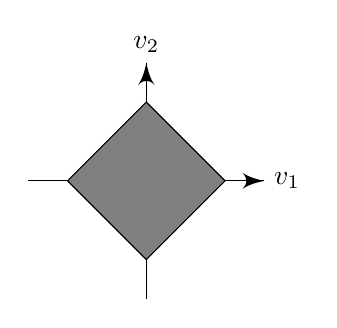
\begin{tikzpicture}
              \draw [->] (-1.5, 0) -- (1.5, 0) node [right] {$v_1$};
              \draw [->] (0, -1.5) -- (0, 1.5) node [above] {$v_2$};
              \draw [fill=gray] (1, 0) -- (0, 1) -- (-1, 0) -- (0, -1) --cycle;
            \end{tikzpicture}
          \end{center}
        \item If $d$ is the metric induced by the $\|\mathbf{v}\|_2 = \sqrt{v_1^2 + v_2^2}$
          \begin{center}
            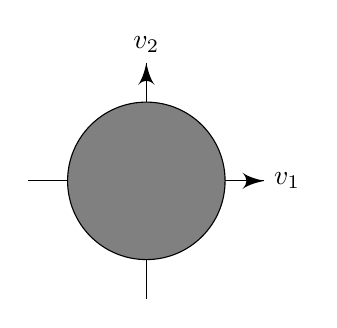
\begin{tikzpicture}
              \draw [->] (-1.5, 0) -- (1.5, 0) node [right] {$v_1$};
              \draw [->] (0, -1.5) -- (0, 1.5) node [above] {$v_2$};
              \draw [fill=gray] circle [radius=1];
            \end{tikzpicture}
          \end{center}

        \item If $d$ is the metric induced by the $\|\mathbf{v}\|_\infty = \max\{|v_1|, |v_2|\}$.
          \begin{center}
            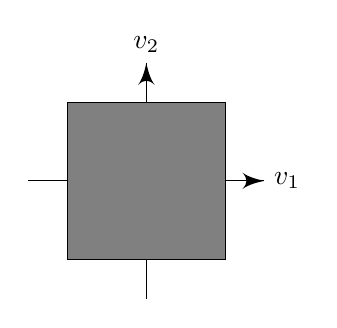
\begin{tikzpicture}
              \draw [->] (-1.5, 0) -- (1.5, 0) node [right] {$v_1$};
              \draw [->] (0, -1.5) -- (0, 1.5) node [above] {$v_2$};
              \draw [fill=gray] (1, 1) -- (1, -1) -- (-1, -1) -- (-1, 1) --cycle;
            \end{tikzpicture}
          \end{center}
      \end{enumerate}
  \end{enumerate}
\end{eg}
\begin{defi}[Open subset]
  $U\subseteq X$ is an \emph{open subset} if for every $x\in U$, $\exists \delta > 0$ such that $B_\delta(x) \subseteq U$.

  $C\subseteq X$ is a \emph{closed subset} if $X\setminus C \subseteq X$ is open.
\end{defi}
This is a very \emph{very} important definition.

We first prove that this makes sense:

\begin{lemma}
  The open ball $B_r(x) \subseteq X$ is an open subset, and the closed ball $\bar{B}_r(x) \subseteq X$ is a closed subset.
\end{lemma}

\begin{proof}
  Given $y\in B_r(x)$, we must find $\delta > 0$ with $B_\delta(y) \subseteq B_r(x)$.
  \begin{center}
    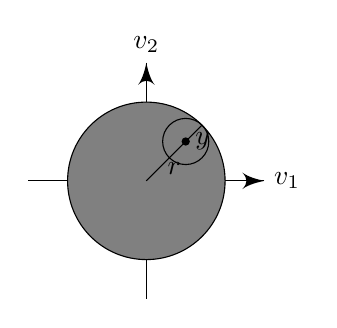
\begin{tikzpicture}
      \draw [->] (-1.5, 0) -- (1.5, 0) node [right] {$v_1$};
      \draw [->] (0, -1.5) -- (0, 1.5) node [above] {$v_2$};
      \draw [fill=gray] circle [radius=1];
      \draw (0, 0) -- (0.707, 0.707) node [below, pos = 0.5] {$r$};
      \draw (0.5, 0.5) node [circ] {} node [right] {$y$};
      \draw (0.5, 0.5) circle [radius=0.293];
    \end{tikzpicture}
  \end{center}

  Since $y\in B_r(x)$, we must have $a = d(y, x) < r$. Let $\delta = r - a > 0$. Then if $z \in B_\delta (y)$, then
  \[
    d(z, x)\leq d(z, y) + d(y, x) < (r - a) + a = r.
  \]
  So $z \in B_r(x)$. So $B_r(y) \subseteq B_r(x)$ as desired.

  The second statement is equivalent to $X\setminus \bar{B}_r(x) = \{y\in X: d(y, x) > r\}$ is open. The proof is very similar.
\end{proof}
\note $A\subseteq X$ is open depends on both $A$ and $X$, not just $A$. For example, $[0, \frac{1}{2}]$ is not an open subset of $\R$, but is an open subset of $[0, 1]$ (since it is $B_{\frac{1}{2}}(0)$), both with the Euclidean metric.

Note also that $A\subseteq X$ can be neither open nor closed. eg. $[0, 1)$ in $\R$ with the Euclidean metric). Also, $\Q\subseteq \R$ is neither open nor closed, since any open interval contains both rational and irrational numbers, and cannot be a subset of $\Q$ or $\R \setminus \Q$.

A subset can also be open \emph{and} close. For example, let $X = [-1, 1]\setminus \{0\}$ with the Euclidean metric. Let $A = [-1, 0)\subseteq X$.. Then $A = B_1(-1)$ and $A = \bar B_{\frac{1}{2}}(-\frac{1}{2})$.

\begin{defi}[Open neighborhood]
  If $x\in X$, an \emph{open neighborhood} of $x$ is an open $U\subseteq X$ with $x\in U$. 
\end{defi}

\begin{lemma}
  If $U$ is an open neighbourhood of $x$ and $x_n \to x$, then $\exists N$ such that $x_n \in U$ for all $n > N$.
\end{lemma}

\begin{proof}
  Since $U$ is open, there exists some $\delta > 0$ such that $B_\delta(x)\subseteq U$. Since $x_n \to x$, $\exists N$ such that $d(x_n, x) < \delta$ for all $n > N$. This implies that $x_n \in B_\delta(x)$ for all $n > N$. So $x_n \in U$ for all $n > N$.
\end{proof}

\begin{defi}[Limit point]
  Let $A\subseteq X$. Then $x\in X$ is a \emph{limit point} of $A$ if there is a sequence $x_n \to x$ such that $x_n \in A$ for all $n$.
\end{defi}

\begin{eg}\leavevmode
  \begin{enumerate}
    \item If $a\in A$, then $a$ is a limit point of $A$, by taking the sequence $a, a, a, a, \cdots$.
    \item If $A = (0, 1)\subseteq \R$, then $0$ is a limit point of $A$, eg. take $x_n = \frac{1}{n}$.
    \item Every $x\in \R$ is a limit point of $\Q$.
  \end{enumerate}
\end{eg}

\begin{prop}
  $C\subseteq X$ is a closed subset if and only if every limit point of $C$ is an element of $C$.
\end{prop}

\begin{proof}
  $(\Rightarrow)$  Suppose $C$ is closed. Then $A = X\setminus C\subseteq X$ is open. Suppose $X$ is a limit point of $C$, so $x_n \to x$, $x_n \in C$ for all $n$.

  Suppose that $x\not\in C$, then $x\in A$, which is open. So by the lemma, we know $\exists N$ such that $x_n \in A$ for all $n > N$. So $x_{N + 1} \in A$ and $x_{N + 1} \in C$, which is a contradiction. So we conclude that $x\in C$.

  $(\Leftarrow)$ Suppose that $C$ is not closed. Then $A$ is not open. So $\exists x\in A$ such that $B_\delta(x)\not\subseteq A$ for all $\delta > 0$. This means that $B_\delta(x) \cap C \not= \emptyset$ for all $\delta > 0$.
  
  So pick $x_n \in B_{\frac{1}{n}}\cap C$ for each $n > 0$. Then $x_n \in C$, $d(x_n, x) = \frac{1}{n} \to 0$. So $x_n \to x$. So $x$ is a limit point of $C$ which is not in $C$.
\end{proof}

Now we come to the Really Important Result\textsuperscript{TM}:
\begin{prop}[Characterization of continuity]
  Let $(X, d_x)$ and $(Y, d_y)$ be metric spaces, and $f: X\to Y$. The following conditions are equivalent:
  \begin{enumerate}
    \item $f$ is continuous
    \item If $x_n \to x$, then $f(x_n) \to f(x)$ (which is the definition of continuity)
    \item For any closed subset $C\subseteq Y$, $f^{-1}(C)$ is closed in $X$.
    \item For any open subset $U\subseteq Y$, $f^{-1}(U)$ is open in $X$.
    \item For any $x\in X$ and $\varepsilon > 0$, $\exists \delta > 0$ such that $f(B_\delta(x)) \subseteq B_\varepsilon(f(x))$, or $d_x(x, z) < \delta \Rightarrow d_y(f(x), f(z)) < \varepsilon$.
  \end{enumerate}
\end{prop}

\begin{proof}\leavevmode
  \begin{itemize}
    \item $1 \Leftrightarrow 2$: by definition
    \item $2 \Rightarrow 3$: Suppose $C\subseteq Y$ is closed, and $x_n \to x$, where $x_n \in f^{-1}(C)$. We want to show that $x\in f^{-1}(C)$.
      
      We have $f(x_n) \to f(x)$ by (2) and $f(x_n) \in C$. So $f(x)$ is a limit point of $C$. Since $C$ is closed, $f(x) \in C$. So $x\in f^{-1}(C)$. So every limit point of $f^{-1}(C)$ is in $f^{-1}(C)$. So $f^{-1}(C)$ is closed.
    \item $3 \Rightarrow 4$: If $U\subseteq Y$ is open, then $Y\setminus U$ is closed in X. So $f^{-1}(Y\setminus U) = X\setminus f^{-1}(U)$ is closed in $X$. So $f^{-1}(U)\subseteq X$ is open.

    \item $4 \Rightarrow 5$: Given $x\in X, \varepsilon > 0$, $B_\varepsilon(f(x))$ is open in $Y$. By (4), $f^{-1}(B_\varepsilon(f(x))) = A$ is open in $X$. Since $x\in A$, $\exists \delta > 0$ with $B_\delta (x) \subseteq A$. So
      \[
        f(B_\delta(x)) \subseteq f(A) = f(f^{-1}(B_\varepsilon f(x))) \subseteq B_\varepsilon (f(x))
      \]
    \item $5 \Rightarrow 2$: Suppose $x_n \to x$. Given $\varepsilon > 0$, $\exists \delta > 0$ such that $f(B_\delta(x)) \subseteq B_\varepsilon(f(x))$. Since $x_n \to x$, $\exists N$ such that $x_n \in B_\delta (x)$ for all $n  > N$ Then $f(x_n) \in f(B(\delta(x))\subseteq B_\varepsilon(f(x))$ for all $n > N$. So $f(x_n) \to f(x)$.
  \end{itemize}
\end{proof}

Note that the third and fourth condition can be useful to decide if a subset is open or closed.

\begin{eg}
  Let $f: \R^3 \to \R$ be defined as
  \[
    f(x_1, x_2, x_3) = x_1^2 + x_2^4 x_3^6 + x_1^8 x_3^2.
  \]
  Then this is continuous. So $\{\mathbf{x}\in \R^3: f(x) \leq 1\} = f^{-1}((-\infty, 1])$ is closed in $\R^3$.
\end{eg}

\begin{lemma}\leavevmode
  \begin{enumerate}
    \item Suppose $V_\alpha \subseteq X$ is open for all $\alpha \in A$. Then $\displaystyle U = \bigcup_{\alpha \in A}V_\alpha$ is open in $X$.
    \item IF $V_1, \cdots, V_n\subseteq X$ are open, then so is $\displaystyle V = \bigcap_{i = 1}^n V_i$.
  \end{enumerate}
\end{lemma}

\begin{proof}\leavevmode
  \begin{enumerate}
    \item If $x\in U$, then $x\in V_\alpha$ for some $\alpha$. Since $V_\alpha$ is open, there exists $\delta > 0$ such that $B_\delta(x) \subseteq V_\alpha$. So $\displaystyle B_\delta (x) \subseteq \bigcup_{\alpha \in A}V_\alpha = U$. So $U$ is open.
    \item If $x\in V$, then $x\in V_i$ for all $i = 1, \cdots, n$. So $\exists \delta_i > 0$ with $B_{\delta_i}(x) \subseteq V_i$. Take $\delta = \min\{\delta_1, \cdots, \delta_n\}$. So $B_\delta(x) \subseteq V_i$ for all $i$. So $B_\delta(x) \subseteq V$. So $V$ is open.
  \end{enumerate}
\end{proof}
\note An infinite intersection of open sets need not be open, eg. the intersection of all $(-\frac{1}{n}, \frac{1}{n})$ is $\{0\}$, which is not open.

\section{Topological spaces}
If $(X, d)$ is a metric space, to decide if $f: X\to Y$ or $g: Z\to X$ are continuous, it's enough to know what the open subsets of $X$ are, and not the metric.

\begin{defi}[Inducing topology]
  Two metrics $d$ and $d'$ on $X$ \emph{induce the same topology} if $U\subseteq X$ is open wrt to $d$ iff $U\subseteq X$ is open wrt to $d'$, ie. they produce the same open subsets.

\end{defi}
If this is true, then $f: (X, d) \to (Y, d_Y)$  is continuous iff $f: (X, d') \to (Y, d_Y)$ is continuous, and $x_n \to x$ wrt $d$ iff $x_n \to x$ wrt $d'$.

\begin{eg}
  Take $X = \R^n$ and $d(\mathbf{x}, \mathbf{y}) = \|\mathbf{x} - \mathbf{y}\|_1$ and $d'(\mathbf{x}, \mathbf{y}) = \|\mathbf{x} - \mathbf{y}\|_\infty$. These induce the same topology:

  $\|\mathbf{v}\| = \sum_{i = 1}^n |v_i|$ and $\|\mathbf{v}\|_\infty = \max_{1 \leq i \leq n}|v_i|$.

  This implies that $\|\mathbf{v}\|_\infty \leq \|\mathbf{v}\|_1 \leq n\|\mathbf{v}\| \infty$.

  So $B_r^\infty(x) \supseteq B_r^1 (x) \supseteq B_{r/n}^\infty$.
  \begin{center}
    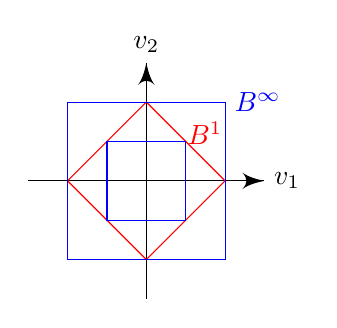
\begin{tikzpicture}
      \draw [->] (-1.5, 0) -- (1.5, 0) node [right] {$v_1$};
      \draw [->] (0, -1.5) -- (0, 1.5) node [above] {$v_2$};
      \draw [red] (1, 0) -- (0, 1) node [pos=0.6, right] {$B^1$} -- (-1, 0) -- (0, -1) -- cycle;
      \draw [blue] (1, 1) -- (1, -1) -- (-1, -1) -- (-1, 1) -- cycle node [right] {$B^{\infty}$};
      \draw [blue] (0.5, 0.5) -- (0.5, -0.5) -- (-0.5, -0.5) -- (-0.5, 0.5) -- cycle;
    \end{tikzpicture}
  \end{center}

  If $U$ is open with respect to $d$, and $x\in U$, then $\exists \delta > 0$ such that $B_\delta^1 (x) \subseteq U$. So $B_{\delta/n}^\infty (x) \subseteq B_\delta^1(x) \subseteq U$.

  Hence $U$ is open with respect to $d'$. The other direction is similar.
\end{eg}

\begin{eg}
  Let $X = C[0, 1]$. If $d(f, g) = \|f - g\|_1$ and $d'(f, g) = \|f - g\|_\infty$, they do not induce the same topology, since $(X, d) \to (X, d')$ by $f\mapsto f$ is not continuous.
\end{eg}

It seems like we can forget about the metrics, and keep the notion of open subsets:
\subsection{Definitions}
Recall that if $X$ is a set, $\P(x) = \{A: A\subseteq X\}$ is the power set of $X$.

\begin{defi}[Topological space]
  A \emph{topological space} is a set $X$ (the space) together with a set $\cU \subseteq \P(X)$ (the topology) such that:
  \begin{enumerate}
    \item $\phi, X\in \cU$
    \item If $V_\alpha\in \cU$ for all $\alpha \in A$, then $\displaystyle \bigcup_{\alpha\in A}V_\alpha \in \cU$.
    \item If $V_1, \cdots, V_n \in \cU$, then $\displaystyle \bigcap_{i = 1}^n V_i \in \cU$.
  \end{enumerate}
  The elements of $X$ are the \emph{points}, and the elements of $\cU$ are the open subsets of $X$.
\end{defi}

\begin{eg}
  If $(X, d)$ is a metric space, then
  \[
    \cU = \{U\subseteq X: U\text{ is open wrt to }d\}
  \]
  is a topology.
\end{eg}

\begin{eg}\leavevmode
  \begin{enumerate}
    \item Let $X$ be any set. 
      \begin{enumerate}
        \item $\cU = \{\phi, X\}$ is the \emph{coarse topology} on $X$.
        \item $\cU = \P(X)$ is the \emph{discrete topology} on $X$, since it is induced by the discrete metric.
        \item $\cU = \{A\subseteq X: X\setminus A\text{ is finite or } A = \emptyset\}$ is the \emph{cofinite topology} on $X$.
      \end{enumerate}
    \item Let $X = \R$, and $\cU = \{(a, \infty): a\in \R\}$ is the \emph{order topology} on $\R$.
  \end{enumerate}
\end{eg}

\begin{defi}[Continuous function]
  If $f: X\to Y$ is a map of topological spaces, $f$ is continuous if $f^{-1}(U)$ is open in $X$ whenever $U$ is open in $Y$.
\end{defi}
\end{document}
